%!TEX root = ../Main.tex

\chapter{Genetic map of \textit{Yr15} with RNA-Seq}
\chaptermark{Genetic map of \textit{Yr15}}
\label{yr15}
%This section describes in detail than the paper of \citet{Ramirez-Gonzalez-2014}
 
%Breeding importance of \textit{Yr15} and original source (an introgression of \textit{T. diccocoides}). 
Wheat breeding programs aim to improve the wheat lines available for production.
One of the traits desired in an elite line is the resistance to pathogens, such as \textit{Puccinia striiformis} f. sp.  \textit{tritici}, the fungi responsible of yellow rust.
A source of resistance genes is are introgressions from other species, such as \textit{Triticum diccocides}. 
In the University of Sydney a collection of \glspl{nil} with introgressions to several Yellow Rust resistance genes on a susceptible background were developed \citep{Wellings1998}. 
On this chapter the NIL for the \textit{Yr15} locus is used to produce a mapping population to improve diagnostic markers. 

%TODO: Paragraph explaining NILs


Line selection can be done with molecular markers that can be used to test if certain allele is present in a line, without the need to do a phenotype.
To find which regions are linked to a trait the use of $F_{2}$ mapping populations is a common practice.
The population is produced by crossing two homozygous parents ($P_1$ and $P_{2}$) with different alleles, A/A (dominant) and a/a (recessive).
When the trait is dominant and has a mendelian segregation, the $F_1$ population show the dominant trait, as it has a copy of each allele (A/a). 
The $F_1$ is then self-crossed to and the population segregates with a ration 1:2:1, dominant:heterozygous:recessive respectively.
This generates a population with a phenotype ratio of 3:1 (dominant:recessive), since the effect of the recessive allele is masked by the dominant gene (\citealt{VanOoijen2013}; Figure \ref{fig:yr15:f2schematic}).  

\begin{SCfigure}
  \centering
    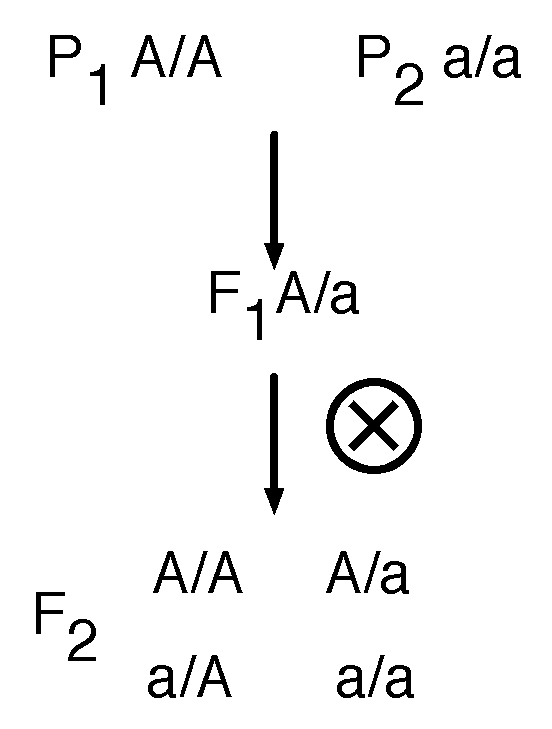
\includegraphics[width=0.4\textwidth]{Yr15/Figures/population/F2schematic.pdf}
  \caption{The cross of two homozygous parents, $P_{1}$ and $P_{2}$, with a dominant and a recessive allele of a gene produce an heterozygous $F_{1}$. The $F_{1}$ crossed with itself produce a segregating $F_{2}$ population with a 1:2:1 ratio (A/A:A/a:a/a). The upper and lower cases represent dominant and recessive alleles  }. 
  \label{fig:yr15:f2schematic}
\end{SCfigure}


\gls{bsa} consists on pooling the DNA of individuals with contrasting phenotypes \citep{Michelmore1991} on a segregating population. 
The bulks show as heterozygous except for the region that is linked to the trait of interest. 
This approach can be used to identify SNPs using High Throughput Sequencing, such as: exome capture \citep{Hodges2007}, RNA-Seq \citep{Pickrell2010}, whole genome resquencing \citep{Schneeberger2009}, among others. 


\begin{figure}
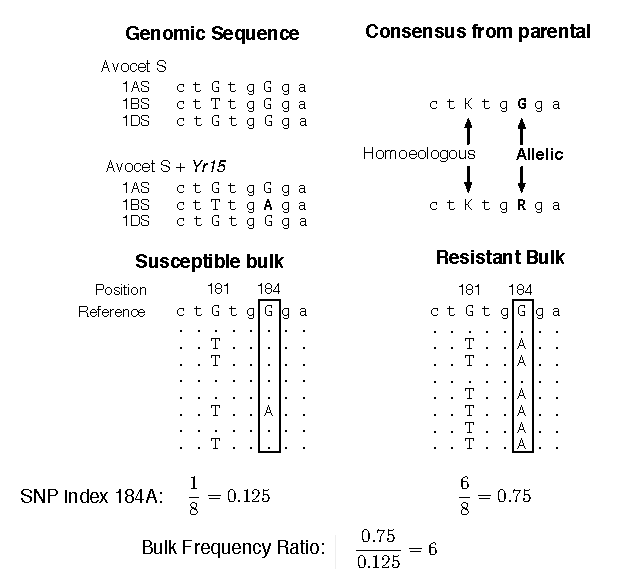
\includegraphics[width=1\textwidth]{Yr15/Figures/bfr.pdf}
\caption{Illustration of a non-informative homoeologous SNP (G181T) present in both parental lines, and an informative allelic SNP (G184A), only present in the resistant progenitor Avocet S + Yr15. The consensus sequences from the parental genotypes include this information in the form of ambiguity codes (K and R, respectively). In the bulks, the individual reads align across the reference sequence, with matches indicated by dots, and polymorphisms at positions 181 and 184 indicated by the corresponding nucleotide variants at those positions. The SNP index is calculated as the frequency of the informative allelic SNP in each bulk. The Bulk Frequency Ratio is the quotient of the resistant and susceptible bulk SNP Indexes. Figure previously published in \citet{Ramirez-Gonzalez2015c}. }
\label{fig:yr15:bfr}
\end{figure}


To Call for SNPs from RNA-Seq a reference transcriptome is used as target when aligning the reads. 
The \gls{bfr} methodology can work on organisms has more than one pseudo genome and that the genes are not necessarily fully characterised independently among homoeologues or paralogues, you can have in a single reference collapsing similar regions. 
The UniGenes database, from NCBI, contains the genes of each species, with all the variations of each gene automatically collapsed and represented as with the longest \acrshort{cdna} \citep{PontiusJUWagnerL2002}. 
The \acrshort{ucw}  genes described in \citet{Krasileva2013} contains 94,177 models from tetraploid and hexaploid wheat, assembled and phased to separate different homoeologues. 
Both gene sets are complement each other, however, the \acrshort{ucw} gene models should provide an improved alignment, since the different homoeologues aren't merged in a single model, a possible side effect of the UniGene pipeline. 

Homoeologous variants, as exemplified by the G$>$T variant at position 181; K in consensus (Figure \ref{fig:yr15:bfr}), will produce the same ambiguity code for both parental consensus sequences and can therefore be excluded. 
Real allelic SNPs between the parental genotypes, exemplified by the G$>$A variant at position 184; R in consensus, are distinguished by the presence in one, but not the other parental consensus sequence. 
The allelic SNPs are then examined further with the alignments of the bulks to identified the SNPs that are enriched on the resistant plants.
The SNP index is the proportion of times an alternative allele is observed over the coverage at certain, in the example the the susceptible bulk has an SNP index of $1/8=0.125$ and $6/8=0.75$ for the resistant bulk \citep{Takagi2013a}. traditional
The \acrshort{bfr} are then calculated by dividing the SNP Index of sample containing the target phenotype (resistance) over the sample without the trait (susceptible), on the example is $0.75/0.125=6$.  
A high BFR suggests that the \acrshort{snp} is linked to the target trait \citep{Trick2012}. 


Finally, the best candidate SNPs where selected to produce a genetic map which lead to a triplet of markers diagnostic to the target locus. 

The steps described in this chapter were first published in \citet{Ramirez-Gonzalez2015c} and the results of this chapter are published in \citet{Ramirez-Gonzalez2015b}.

\section{Mapping population}


\begin{figure}
%\begin{wrapfigure}[17]{R!}{7cm}
    \centering
     
     \begin{subfigure}[b]{0.4\textwidth}
        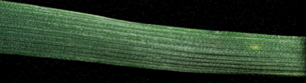
\includegraphics[width=1\textwidth]{Yr15/Figures/population/Yr15Photo.png}
        \caption{}
        \label{fig:yr15.yr15Photo}
    \end{subfigure}
    ~
    \begin{subfigure}[b]{0.4\textwidth}
        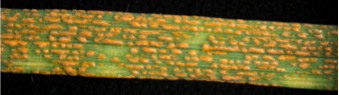
\includegraphics[width=1\textwidth]{Yr15/Figures/population/AVSPhoto.png}
        \caption{}
        \label{fig:yr15:avsPhoto}
    \end{subfigure}

     \begin{subfigure}[b]{0.8\textwidth}
        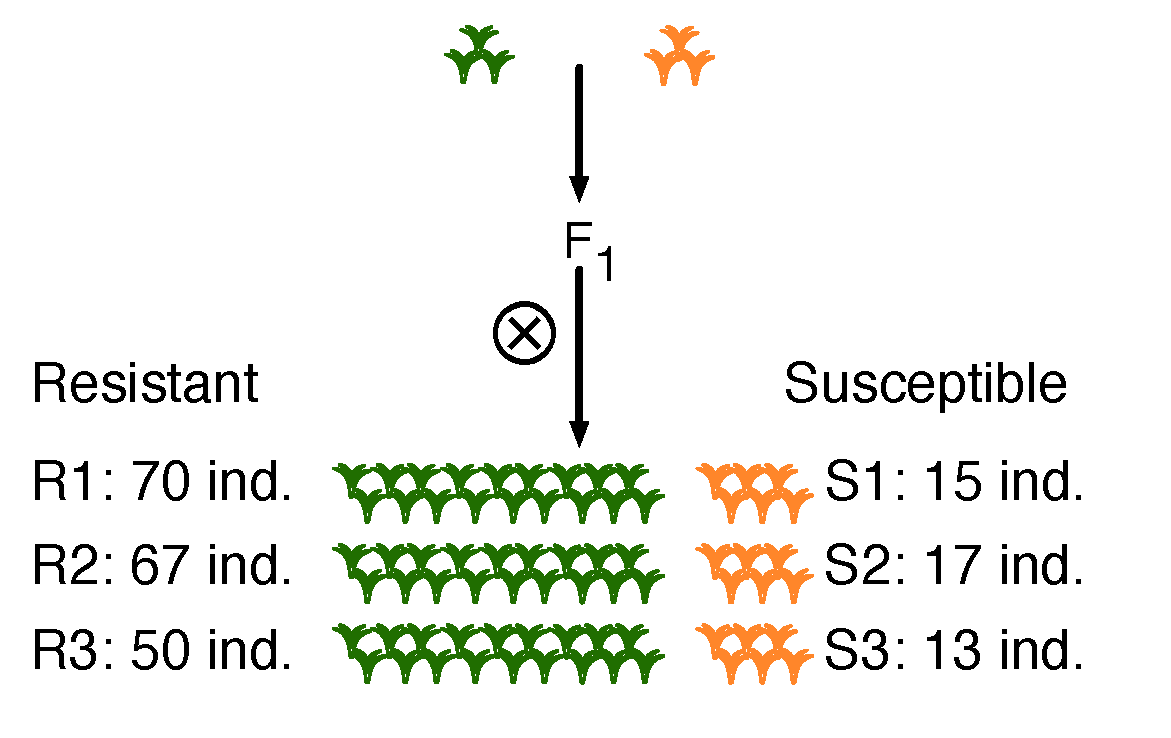
\includegraphics[width=1\textwidth]{Yr15/Figures/population/F2Population.pdf} 
    \caption{ }
    \label{fig:yr15:f2}
	\end{subfigure}

    \caption{Response of (\subref{fig:yr15.yr15Photo}) Avocet + \textit{Yr15} and (\subref{fig:yr15:avsPhoto}) Avocet when inoculated with \textit{Puccinia striiformis} f. sp.  \textit{tritici} at the three leaf stage. (\subref{fig:yr15:f2}) The phenotype of the $F_{2}$ population was used to produce 6 bulks, 3 resistant and 2 susceptible. The RNA was pooled in bulks accordingly. Adapted from \citep{Ramirez-Gonzalez2015b}}

%\end{wrapfigure}
\end{figure}

The population was developed by crossing the resistant line `Avocet + \textit{Yr15}` (\textit{Yr15}) \citep{Wellings1998}, Figure \ref{fig:yr15.yr15Photo}, to the susceptible line Avocet (AVS), Figure \ref{fig:yr15:avsPhoto}. 
$F_{2}$ seeds from tree independent $F_{1}$ plants where sown and tissue was collected, before the fungal inoculation to avoid the effect of the response on the gene expression.  
The plants were challenged at the three leaf stage as it is know that \textit{Yr15} confers resistance in seedlings \citep{Gerechter-Amitai1989}.
The expected segregation on an $F_{2}$ population is 3:1 (resistant:susceptible), since \textit{Yr15} is a dominant gene.
From the 232 plants in the $F_{2}$ population that germinated, 187 were resistant and 45 were susceptible, which deviates slightly from the expected ratio ($\chi^{2}=0.049$).
Segregation distortion has been shown for the same \textit{Yr15} donnor \citep{Randhawa2009}, however the decresed number of succeptible plants can be explained by escapes in the virulence essays (i.e. plants scored as resistant without the \textit{Yr15} locus).   For this study we extracted DNA from individual plants in the $F_{2}$ population and we bulked RNA on 6 different bulks: 3 resistant and, 3 succeptible, Figure \ref{fig:yr15:f2}. 

\section{Sequencing and mapping} 

RNA-Seq was used to avoid sequencing the non-coding regions and reduce the search space.  
The sequencing of the bulks and the parents were done on a single Illumina Hi-Seq2000 each.
The bulks were multiplexed and sequenced on a third of a lane each, as shown on Table \ref{tab:yr15:reads}. 
To ensure that the quality of the sequencencing was good, \verb|fastqc-0.10| \citep{fastqc}  was run with its default parameters in each one of the fastq files.  
The GC content was around 52\% in all the samples (Appendx \ref{App:AppendixQCGC}), which is expected as the sample should be of coding regions, and for wheat the reported GC content in genes is around 55\%.  
The quality of the reads is fairly consistent, in general dropping after the base 80 across the samples (Appendix \ref{App:AppendixQCRead}). 

\begin{table}
\centering
\caption{Arrangement and number of sequenced base pairs per sample. }
\label{tab:yr15:reads}
\begin{tabular}{rrccccc}
\toprule
Library & name & Bar code & Lane   &  Reads (\e{8} bp)\\ 
\midrule
LIB1715 & Bulk R1 & ATCACG & 1 	& 0.77\\
LIB1716 & Bulk R2 & TAGCTT & 1 		& 1.20\\
LIB1717 & Bulk R3 & ACTTGA & 2 	& 0.96  \\ 
LIB1718 & Bulk S1 & GGCTAC & 2 	& 1.64   \\ 
LIB1719 & Bulk S2 & CGTACG & 2 	& 1.49  \\ 
LIB1720 & Bulk S3 & GTGGCC & 1 	&1.88  \\ 
LIB1721 & AvocetS & N/A & 3 		& 4.13 \\ 
LIB1722 & AvocetS + \textit{Yr15} & N/A & 4 	& 3.99  \\ 
\bottomrule
\end{tabular}
\end{table}

%!TEX root = ../../Main.tex
\begin{sidewaystable}
\centering
\caption{Number of genes with a coverage over 20x, 10x and at least one read (\ensuremath{>}0x). }
\label{app:seqAlnCov}
\begin{localsize}{10}{11}

\begin{tabular}{llrrrrrr|rrrr|rr}
\toprule
          &             & \multicolumn{6}{c}{Bulks} & \multicolumn{4}{c}{Bulk  mixes} & \multicolumn{2}{c}{Progenitors}        \\
 Coverage & Reference   & R1     & R2     & R3     & S1     & S2     & S3     & R1+R2       & S1+S2  & R1+R2+R3 & S1+S2+S3 & \textit{Yr15}        & AVS     \\
 \midrule
 20x      & UCW         & 16,434 & 27,871 & 27,223 & 32,287 & 28,669 & 34,898 & 33,968      & 41,019 & 40,985   & 47,507   & 36,808      & 42,248  \\
          &             & 17\%    & 30\%    & 29\%    & 34\%    & 30\%    & 37\%    & 36\%         & 44\%    & 44\%      & 50\%      & 39\%         & 45\%     \\
          & UniGene v60 & 9,643  & 16,182 & 15,222 & 19,549 & 17,397 & 20,567 & 20,219      & 25,270 & 24,598   & 29,052   & 22,107      & 25,842  \\
          &             & 17\%    & 28\%    & 27\%    & 34\%    & 31\%    & 36\%    & 36\%         & 44\%    & 43\%      & 51\%      & 39\%         & 45\%     \\
 \midrule
 10x      & UCW         & 27,371 & 38,282 & 37,777 & 42,658 & 38,999 & 44,610 & 43,266      & 49,473 & 49,182   & 54,781   & 46,356      & 50,760  \\
          &             & 29\%    & 41\%    & 40\%    & 45\%    & 41\%    & 47\%    & 46\%         & 53\%    & 52\%      & 58\%      & 49\%         & 54\%     \\
          & UniGene v60 & 16,201 & 22,948 & 22,130 & 26,200 & 24,130 & 26,914 & 26,318      & 30,579 & 29,857   & 33,557   & 28,044      & 31,095  \\
          &             & 28\%    & 40\%    & 39\%    & 46\%    & 42\%    & 47\%    & 46\%         & 54\%    & 52\%      & 59\%      & 49\%         & 55\%     \\
 \midrule
 \ensuremath{>}0x      & UCW         & 68,302 & 72,484 & 72,957 & 74,694 & 73,290 & 75,201 & 74,397      & 77,093 & 76,715   & 78,796   & 76,275      & 77,080  \\
          &             & 73\%    & 77\%    & 77\%    & 79\%    & 78\%    & 80\%    & 79\%         & 82\%    & 81\%      & 84\%      & 81\%         & 82\%     \\
          & UniGene v60 & 40,717 & 42,489 & 42,595 & 43,625 & 43,059 & 43,748 & 43,393      & 44,655 & 44,364   & 45,392   & 43,732      & 44,596" \\
          &             & 71\%    & 75\%    & 75\%    & 77\%    & 76\%    & 77\%    & 76\%         & 78\%    & 78\%      & 80\%      & 77\%         & 78\%     \\
\bottomrule
\end{tabular}

\end{localsize}
\end{sidewaystable}


When the analysis was started, the draft genome and the corresponding annotation where not not release yet, hence gene models where used. 
All the samples where aligned to the Unigenes v60 (56,954 genes) and the gene models from UCW \citep{Krasileva2013} using \verb|BWA 0.5.9| \citep{Li2009}. 
The alignment provided showed that a few genes were overly expressed, however we still have have 22,107 and 36,808 genes, on the Unigenes and the UCW gene set respectivley,  with a coverage greater than 20x in the progenitor with \textit{Yr15}. 
Both gene sets performed similarly in terms of the percentage of genes with reads and percentage of aligned reads. 
Since each individual bulk has a lower coverage, the susceptible and resistant reads were merged \textit{in silico} as: (i) susceptible bulks 1 with 2 (S1 + S2) and resistant bulks 1 with 2 (R1 + R2) and (ii) all the susceptible (S1 + S2 + S3) and resistant bulks (R1 + R2 + R3). 
The merged samples increased the percentage of genes with coverage over 20x  to 44\% and 50\% in the resistant and susceptible bulks (Table \ref{app:seqAlnCov}), which is close to the coverage from the progenitors.



\section{SNP Calling}


%Using a base coverage threshold of at least 209, we identified SNPs between parental lines and the gene references. Roughly 3% more genes with polymorphisms were identified in AVS compared to Yr15 (Figure 2b) for those genes longer than 500 bp and with at least 50% breadth coverage. This suggests that the lower coverage of Yr15 is affecting the number of putative SNPs identified. Across both parental data sets, the use of the UCW gene models resulted in a higher number of monomorphic genes relative to the UniGene set, leading to a higher SNP frequency in the UniGenes (Figure 2b, Table S3). This is most likely due to the fact that multiple homoeologues are represented as a single sequence within the UniGene set as opposed to the homoeologue-specific UCW set in which a higher percentage of reads map to the correct homoeologues, thereby reducing the number of genes with SNPs. As both references were generated from varieties different to
%AVS and are not complete, we called a base when at least 20% of the reads contained the nucleotide. When more than one putative consensus was identified, the corresponding Interna- tional Union of Pure and Applied Chemistry (IUPAC) ambiguity code was used (Cornish-Bowden, 1985). We next compared SNPs between parental lines; those found in both parents are most likely homoeologous SNP or common varietal polymorphism between AVS and the reference varieties. These shared SNPs are not informative for this study and were thus eliminated from the analysis. On the other hand, SNPs that are unique to a single parent represent putative varietal SNPs and were therefore examined further. Focusing on these unique varietal SNPs, we identified 66 426 putative SNPs across 16 022 UCW genes (17%
The Bulk Frequency Ratio (BFR) algorithm (\citealt{Trick2012}; Figure \ref{fig:yr15:bfr} on tetraploid wheat, was used to identify loci linked to the resistance provided by \textit{Yr15} in the segregating population.
Briefly, the consensus sequence for each of the progenitors is obtained from the pileups, allowing to call variants having 20\% of the bases as an alternative allele. 


\section{\textit{In silico} mapping}
Mapping of the gene models to the IWGSC CSS \citet{Mayer2014} reference and the location of the SNPs using the genetic map from \citet{Wang2014}.

\section{Assay selection}. 
The selection criteria to decide which SNPs where selected to produce the genetic map: BFR$>$6, in the short arm of chromosome group 1 and from the \textit{Yr15} progenitor.

\section{Genetic map} 
\label{yr15:geneticMap}
The three versions of the genetic map: With a subset of the F\textsubscript{2} population

%\section{Assembly of the transcriptome} 
%A comparison between thef known unigenes and the transcript from the progenitors. Since \textit{Yr15} comes from an introgression with \textit{T. diccocoides}, some novel transcripts can be extracted. Analysis of the gels from Mitaly? 

\section{Discussion} 
Remarks on how this techinque can be used to do fine-mapping and that if I were to start the project now I would  use exome capture or Ren-Seq. 

The references have changed since we started
There are new annotations, now we don't necessarily need to use unigenes anymore. 
We can use different techniques now (exome capture, ren-seq)
The markers are now used by our collaborators. 